Les Synapse sont des pairs, qui appartiennent a plusieurs réseaux P2P en même temps. Dans notre exemple ont peut associer cette propriété a un type d'étudiant particulier: \textbf{Les apprentis et les stagiaires.} \\

Le cursus universitaire propose aujourd'hui aux étudiants d'effectuer des stages en entreprise ou même de valider des années en alternances en partageant l'emploi du temps entre l'université et l'entreprise. Ainsi chaque année, l'INRIA accueil des étudiants qui côtoient les chercheurs, enseignants, doctorants et autres ingénieurs experts... 
Ces étudiants remplissent toutes les caractéristiques des synapses, ils appartiennent a la fois au réseau Etudiant et au réseau Entreprise. Dans notre application, ce double statu leur permet d'accéder aux deux réseaux de co-voiturage (avec la même interface). C'est un mécanisme d'invitations similaire aux réseaux sociaux privés qui leur permet de joindre un nouveau réseau. A noter que ce mécanisme n'est pas réservé aux apprentis et aux stagiaires, mais permet a n'importe quel autre membre d'un réseau de devenir synapse, s'il dispose d'une invitation vers un autre réseau.\\

~~~~~~~~~~~~~~~~~~~~~~~~~~~~~ 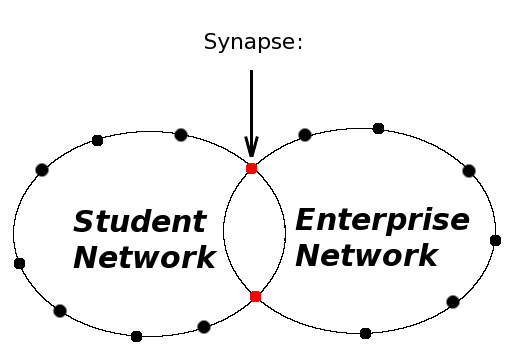
\includegraphics[scale=0.4]{img/schema/Synapse}\\

Les synapses servent de connexion entre ces réseaux hétérogènes. Le protocole décrit précédemment permet de diffuser et de partager les informations entre les différents réseaux. Pour notre application de co-voiturage, le champ "plublic" permet donc de spécifier si l'on souhaite que les informations soit visible ou pas depuis d'autres réseaux.\\
\clearpage
Pour conclure avec notre exemple de l'ingénieur expert qui souhaite faire du co-voiturage, nous voyons que les informations qu'il a publié dans son réseau Entreprise son maintenant visible depuis le réseau Etudiant. Les membres du réseaux Etudiant bénéficient en fait d'une ou plusieurs synapses qui leur permet de propager leurs requêtes de réseaux en réseaux. \\

~~~~~~~~~~~~~~~~~~~~~~~~~~~~~ 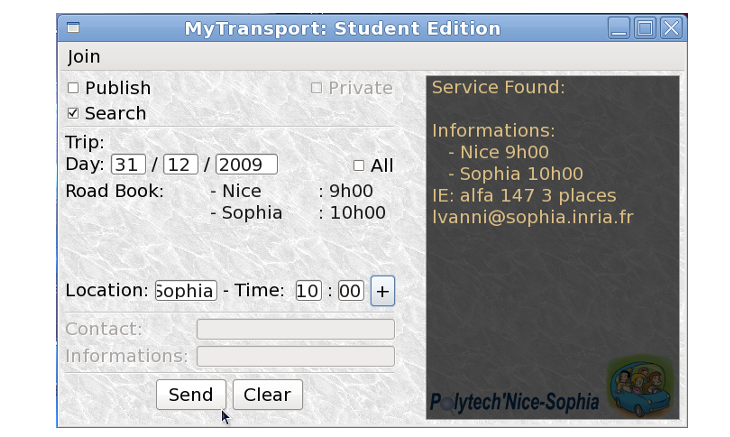
\includegraphics[scale=0.4]{img/screenshot/studentSubFound}\\
